\documentclass[10.5pt,twocolumn]{article}
\usepackage[utf8]{inputenc}
\usepackage[left=0.48in,right=0.48in,top=0.46in,bottom=0.46in]{geometry}
\usepackage{booktabs}
\usepackage{tabularx}
\usepackage{amsmath,amssymb}
\usepackage{hyperref}
\usepackage{enumitem}
\usepackage{xcolor}
\usepackage{microtype}
\usepackage{titlesec}
\usepackage{graphicx}
\usepackage{tikz}
\usetikzlibrary{shapes.geometric,arrows.meta,positioning,calc,fit,backgrounds}

% Ultra-compact styling to guarantee 2-page cutoff
\titlespacing*{\section}{0pt}{3pt plus 1pt minus 0.5pt}{1pt plus 0.5pt minus 0.5pt}
\titlespacing*{\subsection}{0pt}{2pt plus 0.5pt minus 0.5pt}{0.8pt plus 0.5pt minus 0.5pt}
\setlist{nosep,leftmargin=1.1em,itemsep=0.5pt}
\setlength{\parskip}{0pt}
\hypersetup{colorlinks=true,linkcolor=blue!75!black,urlcolor=blue!75!black}

\title{\vspace{-22pt}\textbf{\Large Pixarch: On-Device Photo Retrieval Pipeline}\\[1pt]\large Project Mid Report\vspace{-7pt}}
\author{
  \textbf{Team: Paisaan}\\[2pt]
  \textbf{Shivam Patel} (2025202030) \quad
  \textbf{Suyash Pande} (2025201063) \quad
  \textbf{Kavan Gandhi} (2025201078)\\[1pt]
%   \textit{International Institute of Information Technology, Hyderabad (IIIT-H)}
}
\date{}

\begin{document}
\maketitle

\section{Introduction \& Project Overview}
\textbf{Pixarch} is an on-device personal data retrieval system that indexes personal photos, documents, receipts, and scans entirely on-device with zero cloud offloading. The system processes multimodal personal data via a split-branch architecture: OCR with inverted indexing (BM25) for documents, and vision-language vector embeddings for scenes. This report details progress on corpus construction, baseline architecture, model selection for desktop simulation vs. edge deployment, empirical benchmark evaluations, and the next-stage roadmap.

\section{Labeled Dataset Creation}
Personal device storage exhibits extreme modality imbalance: camera photos, noisy document scans, identity cards, financial records, and digital receipts. To simulate realistic device storage, a balanced, labeled corpus of \textbf{629 images} (627 unique indexed; 2 duplicate receipts resolved) was constructed across \textbf{31 subtypes} (14 document, 17 scene):

\begin{itemize}
    \item \textbf{Document Bucket (289 items, 14 categories):} Aadhaar (24), PAN (21), DL (22), Passport (22), Bank Statement (20), Passbook (20), Credit Card (20), Debit Card (20), Bill (20), Receipt (20), Report Card (20), Book (20), IAM Handwritten Page (20), and General Doc (20).
    \item \textbf{Scene Bucket (340 items, 17 categories, 20 each):} Beach, Mountain, Trees, Food, Fitness, Wedding, Party, Travel, Planes, Transit Hub, Mall, College, Clothes, Art, Outdoor Games, Vehicle, and X-ray.
\end{itemize}

\subsection{Sourcing and Annotation Methodology}
The dataset combines authentic open benchmarks with privacy-preserving synthetic specimens:
\begin{enumerate}
    \item \textbf{Public Benchmarks (449 items):} SROIE (ICDAR 2019) for receipts with upstream word-level OCR ground truth; IAM Handwriting lines assembled into full pages; SUN397 dataset (via HF datasets server) across 10 scene categories; and Wikimedia Commons public identity card specimens.
    \item \textbf{Privacy-Preserving Synthetics (180 items):} Realistically rendered Indian identity cards, passbooks, and statements preserving true typography and layout without exposing real PII.
    \item \textbf{Ground Truth \& Judgments:} A master manifest (\texttt{manifest.csv}) tracks SHA-256 hashes, source URLs, licenses, dimensions, and subtype labels. A test suite of \textbf{98 user queries} (\texttt{queries.jsonl}) covering all 31 subtypes was expanded into \textbf{2,183 graded relevance judgments} (\texttt{qrels.csv}).
\end{enumerate}

\section{Models Used for PC Simulation}
The desktop simulation verifies algorithmic plumbing and provides a rigorous performance baseline:
\begin{itemize}
    \item \textbf{Vision-Language Representation (CLIP):} \texttt{ViT-B-32} pre-trained on \texttt{laion2b\_s34b\_b79k} via OpenCLIP. Reused dual-purpose: zero-shot document/scene routing and 512-dimensional float32 scene embeddings.
    \item \textbf{Text Recognition (OCR):} Pure \textbf{Tesseract OCR (v5.x)} with English language pack (\texttt{eng}). Extracts bounding boxes, confidences ($\ge 30$), and normalized text tokens without external post-processing pipelines.
    \item \textbf{Inverted Index \& BM25 Ranking:} \textbf{SQLite FTS5}. Integrates full-text inverted indexing with native Okapi BM25 scoring and column weighting ($1\times$ OCR body text, $5\times$ document subtype tags).
    \item \textbf{Vector Store:} Exact cosine similarity matrix multiplication over L2-normalized vectors stored in SQLite.
\end{itemize}

\section{Finalized Models for Edge Device (Android)}
For edge deployment (Android smartphone), model selections must satisfy strict memory limits ($<150$\,MB), zero cloud dependencies, low latency, and battery efficiency:
\begin{itemize}
    \item \textbf{On-Device Multimodal Encoder:} \textbf{MobileCLIP} (\texttt{MobileCLIP-S0} / \texttt{S2}) or quantized TFLite/ONNX-Runtime MobileCLIP. Replaces ViT-B-32 with a lightweight footprint ($<40$\,MB), delivering $4\times$ faster NPU inference with minimal zero-shot degradation.
    \item \textbf{On-Device OCR Engine:} \textbf{Google ML Kit Text Recognition v2}. Shipped natively via Android Play Services; executes on-device without model bundling bloat, offering hardware-accelerated Latin and Devanagari recognition at $<100$\,ms/frame.
    \item \textbf{Storage \& FTS Index:} Native \textbf{Android SQLite FTS5}. Zero dependency overhead; exact schema and BM25 parity with desktop simulation.
    \item \textbf{Vector Search Seam:} Lightweight BLOB vector scan or \textbf{usearch / ObjectBox} embedded vector store for sub-millisecond on-device similarity search.
\end{itemize}

\section{Baseline Architecture}
The baseline implements a single-shot, un-fused pipeline as illustrated in Figure~\ref{fig:arch}:
\begin{enumerate}
    \item \textbf{Stage 0 (Ingest):} Computes SHA-256 for de-duplication, parses EXIF metadata, and flags screenshots via aspect ratio heuristics.
    \item \textbf{Stage 1 (Classification):} Zero-shot scoring against document vs. scene prompt prototypes. Margin $<0.05$ hedges items into \textit{both} branches.
    \item \textbf{Stage 2a (Document Branch):} Pure Tesseract OCR extracts text blocks $\rightarrow$ rule-based subtype tagging $\rightarrow$ indexed into SQLite FTS5.
    \item \textbf{Stage 2b (Scene Branch):} 512-dim visual embeddings stored in SQLite vector store.
    \item \textbf{Stage 3 (Query Routing):} Lexical rules classify intents ($>95\%$ accuracy) with CLIP semantic fallback, directing queries to FTS5 (BM25) or Vector Search.
\end{enumerate}

\begin{figure}[htbp]
\centering
\resizebox{\columnwidth}{!}{%
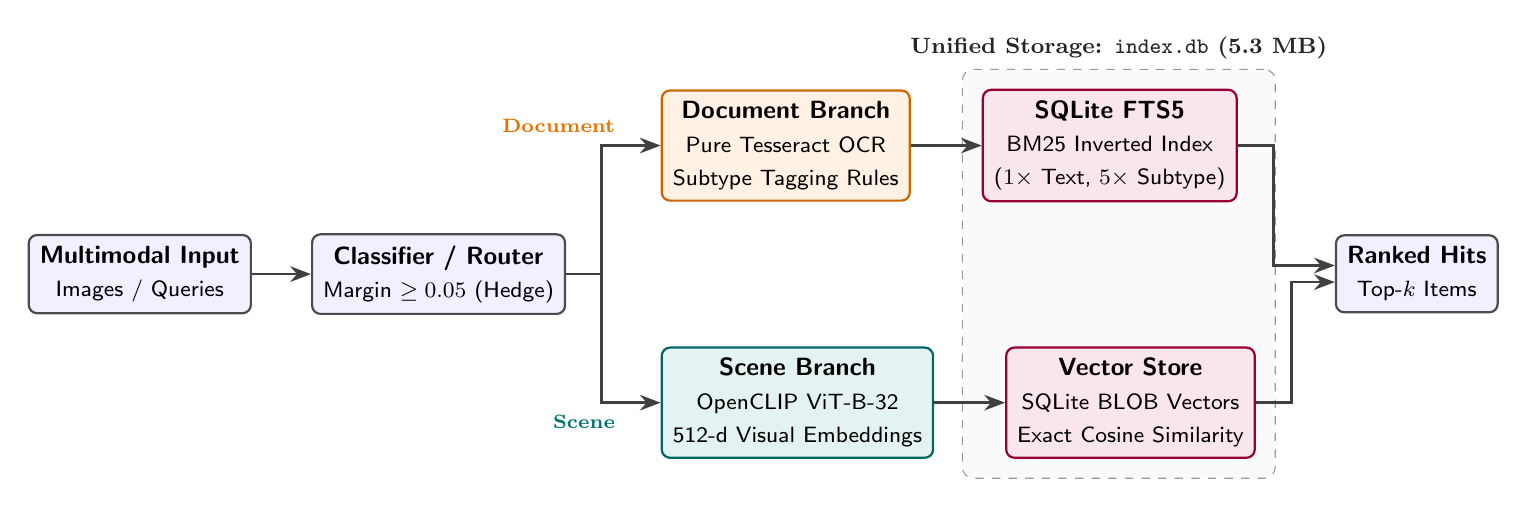
\begin{tikzpicture}[
    font=\sffamily\small,
    >=Stealth,
    thick,
    node distance=0.55cm and 0.8cm,
    block/.style={draw=black!70, rounded corners=3pt, fill=blue!6, align=center, inner sep=4pt, line width=0.8pt},
    docblock/.style={draw=orange!80!black, rounded corners=3pt, fill=orange!10, align=center, inner sep=4pt, line width=0.8pt},
    scnblock/.style={draw=teal!80!black, rounded corners=3pt, fill=teal!10, align=center, inner sep=4pt, line width=0.8pt},
    dbblock/.style={draw=purple!80!black, rounded corners=3pt, fill=purple!10, align=center, inner sep=4pt, line width=0.8pt},
    groupbox/.style={draw=black!40, dashed, rounded corners=4pt, fill=black!2, inner sep=7pt},
    arrow/.style={->, line width=1pt, draw=black!75}
]

% Inputs
\node[block] (input) {\textbf{Multimodal Input}\\[1pt]\footnotesize Images / Queries};

% Router / Classifier
\node[block, right=0.75cm of input] (router) {\textbf{Classifier / Router}\\[1pt]\footnotesize Margin $\ge 0.05$ (Hedge)};

% Document Branch (Top)
\node[docblock, above right=0.4cm and 1.2cm of router] (ocr) {\textbf{Document Branch}\\[1pt]\footnotesize Pure Tesseract OCR\\[1pt]\footnotesize Subtype Tagging Rules};

% Scene Branch (Bottom)
\node[scnblock, below right=0.4cm and 1.2cm of router] (clip) {\textbf{Scene Branch}\\[1pt]\footnotesize OpenCLIP ViT-B-32\\[1pt]\footnotesize 512-d Visual Embeddings};

% Unified Storage (index.db)
\node[dbblock, right=0.9cm of ocr] (fts) {\textbf{SQLite FTS5}\\[1pt]\footnotesize BM25 Inverted Index\\[1pt]\footnotesize ($1\times$ Text, $5\times$ Subtype)};

\node[dbblock, right=0.9cm of clip] (vec) {\textbf{Vector Store}\\[1pt]\footnotesize SQLite BLOB Vectors\\[1pt]\footnotesize Exact Cosine Similarity};

% Unified DB Container background
\begin{scope}[on background layer]
  \node[groupbox, fit=(fts) (vec), label={[font=\footnotesize\bfseries, text=black!85]above:Unified Storage: \texttt{index.db} (5.3 MB)}] (dbbox) {};
\end{scope}

% Output clearly to the right of the dbbox container
\node[block, right=0.75cm of dbbox.east] (output) {\textbf{Ranked Hits}\\[1pt]\footnotesize Top-$k$ Items};

% Arrows
\draw[arrow] (input) -- (router);

% Route fork with labels clearly placed above/below the horizontal branch
\draw[arrow] (router.east) -- ++(0.45,0) |- (ocr.west) node[pos=0.72, above left=1pt, font=\scriptsize\bfseries, text=orange!90!black] {Document};
\draw[arrow] (router.east) -- ++(0.45,0) |- (clip.west) node[pos=0.72, below left=1pt, font=\scriptsize\bfseries, text=teal!90!black] {Scene};

\draw[arrow] (ocr) -- (fts);
\draw[arrow] (clip) -- (vec);

% Arrows from FTS / Vector Store into Output
\draw[arrow] (fts.east) -- ++(0.45,0) |- ([yshift=3pt]output.west);
\draw[arrow] (vec.east) -- ++(0.45,0) |- ([yshift=-3pt]output.west);

\end{tikzpicture}%
}
\caption{Pixarch Dual-Branch Baseline Architecture.}
\label{fig:arch}
\end{figure}

\section{Results \& Performance Benchmarks}
\textit{Platform Note:} Currently, all benchmark results were conducted on \textbf{PC simulation} (desktop environment). The next stage of development will focus on implementing and evaluating these models directly on an \textbf{edge device} (Android smartphone).

\subsection{Information Retrieval Performance}
Evaluated across 98 queries over 627 indexed items (retrieval depth 107). Table~\ref{tab:retrieval} compares the Routed Baseline against single-model comparators.

\begin{table}[htbp]
\centering
\scriptsize
\setlength{\tabcolsep}{2.0pt}
\begin{tabular}{lcccccc}
\toprule
\textbf{System} & \textbf{P@1} & \textbf{P@5} & \textbf{MRR@10} & \textbf{nDCG@10} & \textbf{R-prec} & \textbf{R@10} \\
\midrule
\textbf{Routed Baseline} & \textbf{0.773} & \textbf{0.781} & \textbf{0.803} & \textbf{0.773} & \textbf{0.693} & \textbf{0.369} \\
CLIP-only & 0.629 & 0.596 & 0.644 & 0.580 & 0.478 & 0.278 \\
BM25-only & 0.361 & 0.355 & 0.378 & 0.349 & 0.312 & 0.157 \\
\bottomrule
\end{tabular}
\caption{Retrieval effectiveness vs. single-model comparators (98 queries).}
\label{tab:retrieval}
\end{table}

\textbf{Routing Value \& Recall Ceilings:} Routing beats both single-model comparators overall (+0.144 P@1 over CLIP-only; +0.412 over BM25-only). Single-model systems collapse on opposing domains: BM25 scores 0.020 on scenes; CLIP scores 0.370 on documents. Macro-averaged P@1 across buckets highlights routing robustness: Routed (\textbf{0.772}) tracks the upper bound, while CLIP-only drops to 0.616 and BM25-only to 0.379. With $\sim$20 relevant items per subtype, Recall@10 caps at 0.480; the baseline achieves \textbf{77.0\% of achievable recall} (0.369/0.480) and \textbf{0.693} R-precision.

\subsection{Ingestion Cost \& Throughput}
Full corpus indexing of 627 items completed in 352.4\,s on PC (\textbf{1.78 images/sec} end-to-end throughput).

\begin{table}[htbp]
\centering
\scriptsize
\setlength{\tabcolsep}{2.0pt}
\begin{tabular}{lrrrr}
\toprule
\textbf{Stage} & \textbf{Items} & \textbf{Time (s)} & \textbf{ms/image} & \textbf{Throughput} \\
\midrule
0. Ingest & 627 & 18.2 & 29.1\,ms & 34.41\,img/s \\
1. CLIP Encode & 627 & 27.1 & 43.2\,ms & 23.14\,img/s \\
1b. Routing/Classify & 627 & 16.9 & 26.9\,ms & 37.22\,img/s \\
2b. Embed Store & 627 & 0.1 & 0.2\,ms & 4209.58\,img/s \\
2a. Tesseract OCR & 393 & 290.0 & 738.0\,ms & 1.35\,img/s \\
\midrule
\textbf{End-to-End Pipeline} & \textbf{627} & \textbf{352.4} & \textbf{562.0\,ms} & \textbf{1.78\,img/s} \\
\bottomrule
\end{tabular}
\caption{Ingestion pipeline stage timings and throughput.}
\label{tab:ingest}
\end{table}

\textbf{Throughput Bottleneck:} OCR constitutes \textbf{82\%} of total indexing time, making documents $\sim$11$\times$ more expensive than scenes (scene: 10.06\,img/s; doc: 0.90\,img/s). A 10,000-item gallery projects to 1.56 hours indexing on desktop GPU.

\subsection{Query Latency}
Evaluated across warm sequential benchmark queries ($n=98$):
\begin{itemize}
    \item \textbf{Routed Document:} Mean \textbf{4.1\,ms}, p50 \textbf{1.6\,ms}, p95 \textbf{8.5\,ms}, max 46.9\,ms.
    \item \textbf{Routed Scene:} Mean \textbf{11.9\,ms}, p50 \textbf{12.4\,ms}, p95 \textbf{15.2\,ms}, max 63.3\,ms.
    \item \textbf{Overall Queries:} Mean \textbf{8.0\,ms}, p50 \textbf{6.8\,ms}, p95 \textbf{13.5\,ms}, max 63.3\,ms.
\end{itemize}

\subsection{Module Benchmarks \& Storage}
\begin{itemize}
    \item \textbf{Bucket Classification (CLIP Zero-Shot):} \textbf{98.6\%} accuracy (618/627 correct; 8 scene $\rightarrow$ doc, 1 doc $\rightarrow$ scene).
    \item \textbf{Query Routing Accuracy:} \textbf{95.9\%} (94/98 correct; 3 misrouted are X-rays, 1 intentionally ambiguous).
    \item \textbf{Subtype Tagging (\texttt{doctype.py}):} \textbf{70.7\%} overall (100\% on synthetic; 21.5\% on photographed documents).
    \item \textbf{Tesseract OCR Accuracy (258 items):} Overall CER = \textbf{0.471}, WER = \textbf{0.596}; excluding bill: CER = \textbf{0.420}, WER = \textbf{0.527} (synthetic CER 0.418 vs. fetched 0.592).
    \item \textbf{Storage Footprint:} \texttt{index.db} is \textbf{5.3\,MB} ($\approx$\textbf{8.5\,KB/image}; embeddings 48.3\%, OCR blocks 28.9\%, inverted index 6.7\%). Projected 10k items gallery is \textbf{85\,MB}.
\end{itemize}

\section{Next Stage Development \& Roadmap}
Building upon the established PC baseline, the upcoming phase focuses on edge porting, quality refinement, and interaction extensions:
\begin{enumerate}
    \item \textbf{Mobile Device Implementation:} Deploying the full pipeline on Android using Google ML Kit Text Recognition v2 and quantized MobileCLIP (FP16/INT8), optimizing on-device memory footprints and battery efficiency.
    \item \textbf{Pre-OCR Image Processing:} Introducing adaptive binarization, skew correction, and contrast normalization prior to OCR to enhance character recognition on noisy and mobile-captured scans.
    \item \textbf{Document Semantic Search \& Tradeoffs:} Integrating dense neural document embeddings alongside BM25, measuring on-device latency vs. retrieval recall tradeoffs.
    \item \textbf{Query Rewriting:} Implementing lightweight local query expansion to resolve ambiguous terms and improve intent routing.
    \item \textbf{OCR Correction via \texttt{ocrfixr}:} Evaluating the feasibility and latency overhead of running token repair (\texttt{ocrfixr}) on mobile hardware to fix corrupted OCR text.
    \item \textbf{Image-Conditioned Multimodal Search:} (Time permitting) Supporting image-plus-query search (e.g., \textit{``find images with similar background''}).
\end{enumerate}

\section{Source Code Repository}
The complete reproducible codebase, configuration files, manifests, test suites, and evaluation scripts are available at:
\begin{center}
\small\url{https://github.com/shivam-git-acc/Pixarch}
\end{center}

\end{document}
